
%%%%%%%%%%%%%%%%%%%%%%%%%%%%%%%%%%%%%%%%%%%%%%%%%%%%%%%%%%%%%%%%%%%%%%%%%%%%%%%
%     STYLE POUR LES EXPOSÉS TECHNIQUES 
%         3e année INSA de Rennes
%
%             NE PAS MODIFIER
%%%%%%%%%%%%%%%%%%%%%%%%%%%%%%%%%%%%%%%%%%%%%%%%%%%%%%%%%%%%%%%%%%%%%%%%%%%%%%%

\documentclass[a4paper,11pt]{article}
\usepackage[dvips]{graphicx}
\usepackage[T1]{fontenc}
\usepackage[utf8]{inputenc}
\usepackage[french]{babel}
\usepackage{lmodern} \normalfont
\DeclareFontShape{T1}{lmr}{bx}{sc}{<-> ssub * cmr/bx/sc}{}
\usepackage{textcomp}
\usepackage{fixltx2e}
\usepackage{exptech} % inclusion du style immposé
\usepackage{amsmath}
\usepackage{amssymb}
\usepackage{graphicx}
\usepackage{wrapfig}
\usepackage{subcaption}
\usepackage{listings}
\usepackage{setspace}
\usepackage{color}
\usepackage{pdfpages}
\usepackage[colorlinks=true,
			linkcolor=blue,
			bookmarksnumbered=true,
			pdftitle={Report},
			pdfauthor={Julien B.},
			pdfborder={0 0 0},
			pdfsubject={mittelwerk}]{hyperref}


\title{\textbf{Contrôleurs dans l'espace: Documentation utilisateur}}
\author{Julien \textsc{Bouvet}, Antoine \textsc{Chenon}, Mikaïl \textsc{Demirdelen}, Hoel \textsc{Kervadec}
        \\
        Encadrants : Yann \textsc{Ricquebourg}, Loic \textsc{Helouet}}
\date{Juin 2014}
\markright{Contrôleurs dans l'espace}


\thispagestyle{empty}

%%%%%%%%%%%%%%%%%%%%%%%%%%%%%%%%%%%%%%%%%%%%%%%%%%%%%%%%%%%%%%%%%%%%%%%%%%%%%%%

\begin{document}          
\onehalfspacing
\maketitle
%%%%%%%%%%%%%%%%%%%%%%%%%%%%%%%%%%%%%%%%%%%%%%%%%%%%%%%%%%%%%%%%%%%%%%%%%%%%%%%           
\section{Avant-propos}

\begin{figure}[!h]
            \begin{center}
                
\includegraphics[width=0.7\textwidth]{img/orbiter_logo.png}
            \end{center}
\end{figure}

\subsection{Un simulateur en temps réel}

Orbiter est un simulateur de vol spatial, créé par Dr. Martin Schweiger en 2000 et ce afin de combler le manque de simulateur de vol réaliste disponible sur internet. Gratuit mais non libre, un kit de développement a fait son apparition pour permettre à tout un chacun de développer son propre vaisseau. Fourni avec un lot de scénarios et de vaisseaux, Orbiter permet d'expérimenter et de mieux appréhender les lois de la physique.

C'est dans cette optique que nous proposons une première démarche d'automatisations des vaisseaux dans Orbiter.

Dans un premier temps ce projet est compatible avec un seul vaisseau : le ShuttleA.

\subsection{Module lunaire}

Le ShuttleA est un module lunaire : en effet il est conçu pour permettre aux spationautes de rentrer sur Terre une fois l'alunissage terminé. Ses caractéristiques sont donc plus adaptées à cet environnement. En effet le décollage depuis la Terre est plus diffcile (compte tenu de la gravité, plus forte que sur la Lune) et plus gourmand en carburant. Cependant le ShuttleA a deux avantages :

\begin{itemize}
	\item Il dispose de nombreux propulseurs, ce qui en facilite la manoeuvre
	\item Il est codé en une seule classe C++ : c'est transparent pour l'utilisateur, mais dans le cas de notre travail, cela simplifie grandement l'étude.
\end{itemize}


\subsection{Théorie du contrôle}
Pour pouvoir automatiser le pilotage des vaisseau, en particulier du ShuttleA nous disposons de plusieurs outils formels, dont la théorie du contrôle.

C'est un moyen de formaliser le fait qu'un système, pour se maintenir sur une trajectoire prend des mesures, les compare à des références et corrige si nécessaire. C'est une boucle qui va des capteurs vers le contrôleur, chargé de prendre les décisions pour suivre l'objectif.

\begin{figure}[!h]
            \begin{center}
                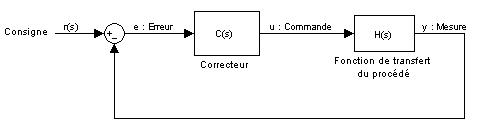
\includegraphics[width=0.7\textwidth]{img/boucle_controle.jpg}
            \end{center}
\end{figure}

\subsection{Automates}
Les automates sont un ensemble d'états et de transitions, qui correspondent à des états d'un système. Par exemple on peut imaginer qu'une lampe soit modélisée par un automate. Elle aurait deux états : Allumée, éteinte. Cette lampe peut passer d'un état à l'autre grâce à des transitions.
Ces transitions définissent sous quelles conditions le système change d'état.
Pour la lampe, la transition de l'état éteinte vers allumée se fait par exemple si elle est alimentée et vice-versa.

\begin{figure}[!h]
            \begin{center}
                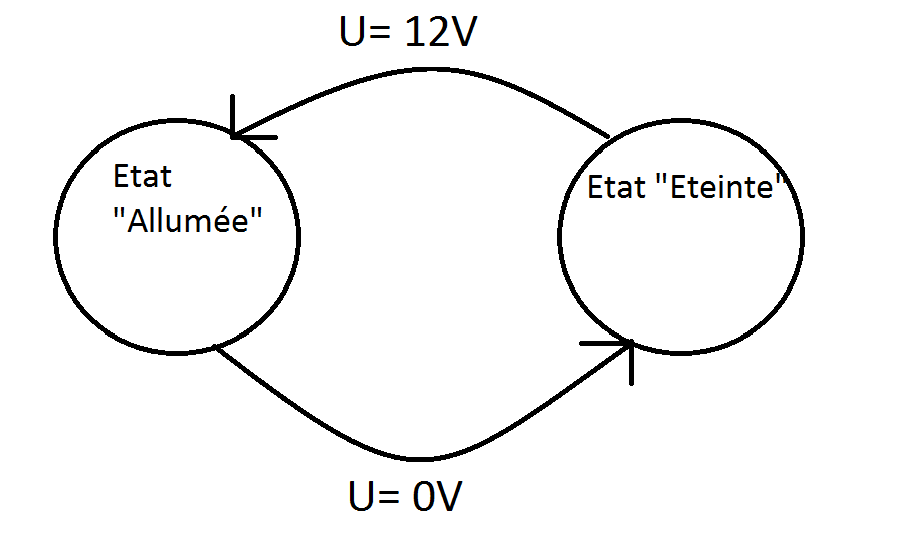
\includegraphics[width=0.7\textwidth]{img/automatelas.png}
            \end{center}
\end{figure}

Pour le vaisseau on peut imaginer une infinité d'états différents, ce qui permet de contrôler le vaisseau à notre guise. Par exemple l'état "Propulsion MAXI" avec une transition sur l'état "Propulsion Gauche seule" en cas de détection d'obstacle.

%%%%%%%%%%%%%%%%%%%%%%%%%%%%%%%%%%%%%%%%%%%%%%%%%%%%%%%%%%%%%%%%%%%%%%%%%%%%%%%
\section{Langage Mittlewerk}

\subsection{Introduction}
Nous avons créé un langage simple permettant de piloter le vaisseau sans maîtriser le C++. En effet, ce langage permet de créer facilement des automates, et donc de créer un contrôleur personnalisé.
Certains aspects du langage sont proches du C++ mais ce sont des concepts classiques en programmation (affectation, déclaration ...).

\subsection{Instructions basiques}
Toutes les instructions se terminent par un ';' pour indiquer au compilateur qu'une instruction est complète.

\subsubsection{Variables}

Une variable a un nom et un type, il faut donc les déclarer au compilateur avant de pouvoir les utiliser. Cela se fait très simplement : 
\begin{center}
\texttt{type nom;}
\end{center}
\textit{\textbf{Attention :} les variables doivent être toutes déclarées au début de la fonction avant d'autres instructions.} 

\newline
\textit{\textbf{Remarques :}} 
\textit{\begin{itemize}
	\item les variables peuvent être déclarés en groupe si elles sont du même type : \texttt{DOUBLE a, b, c;}
	\item Des valeurs t, dt et mjd sont accessibles. t correspond au temps écoulé pendant la simulation en secondes, dt est l'intervalle de temps entre deux calculs de simulation : dt est donc le pas de la simulation. Enfin mjd correspond à t mais exprimée dans le calendrier Julien, permettant si la simulation dure très longtemps (aller-retour sur mars) d'exprimer la valeur autrement qu'en secondes !
\end{itemize}}
 


Par exemple, si vous souhaitez définir un double (nombre à virgule à valeur max très élevée) que vous appelez toto, il faudra l'avoir défini avant de l'utiliser : 
\begin{center}
\texttt{DOUBLE toto;}
\end{center}
\textit{\textbf{Attention : }n'utilisez pas de caractères spéciaux, ni accentués, ni espaces dans les noms de fonctions et variables. Ne nommez pas non plus vos variables t, dt ou mjd.}

Pour affecter une valeur, la démarche est identique à la plupart des langages :
\begin{center}
	\texttt{toto = 42;}
	
	\texttt{toto = toto + 1;}
	
	\texttt{toto = max(1, toto);}
\end{center}
On peut affecter à une variable la valeur de retour d'une fonction, d'une autre variable ... Il faut juste vérifier que le type que l'on donne à la variable correspond à celui qu'on lui a donné lors de sa déclaration.
Les types disponibles sont BOOL (TRUE ou FALSE), INT, DOUBLE.

\subsubsection{Fonctions}
Les fonctions peuvent être déclarées, hors du corps d'une fonction, et être appelées, dans le corps d'une fonction ou dans un etat de l'Automate.

Pour déclarer une fonction c'est très simple : 
\begin{center}
\texttt{type nomDeFonction(type1 Param1, type2 Param2 ...) \{ corps de la fonction \}}
\end{center}


Si la fonction a un type différent de VOID, elle doit retourner une valeur : 
\begin{center}
\texttt{RETURN toto;}
\end{center}

Pour l'appeler : \texttt{ nomDeFonction(param1, param2, ...)}

\subsubsection{Commentaires}
Il est parfois très utile de commenter son code : ce qui est commenté n'est pas interpreté lors de la compilation, ce ne sont que des informations pour les humains.
Pour encadrer du commentaire il faut mettre /* avant le commentaire, */ à la fin.
\begin{center}
\texttt{VOID fonctionInutile() \{ /* cette fonction ne fait rien*/ \}}
\end{center}

\subsubsection{Opérateurs de base}

Sur les \textsc{bool} : 
\begin{itemize}
	\item == teste l'égalité booléenne
	\item != teste la différence booléenne 
	\item OR renvoie \textsc{true} si un (au moins) des booléens est vrai
	\item AND renvoie \textsc{true} si les deux booléens sont vrais, \textsc{false} sinon
\end{itemize}

Sur les \textsc{double} ou \textsc{int} tous les opérateurs classiques :
\begin{itemize}
	\item Opérateurs mathématiques : +,*,-,/
	\item Opérateurs de test : ==, !=, <, <=, >, >=
\end{itemize}

\subsubsection{Structure de test}
 Là encore, le mécanisme est un grand classique. Pour tester si une condition est vraie et faire une action en conséquence, on utilise une structure \textsc{if} ... \textsc{else} :

\texttt{\textsc{if} (condition) \{Action si condition = TRUE\}}

\texttt{\textsc{else}  \{Action si cond = FALSE\}}

\textit{\textbf{Remarques : }
\begin{itemize}
	\item Condtition doit être de type \textsc{bool}.
	\item Pas de ';' après '\}', if et else ne sont pas des intructions. Par contre à l'intérieur des accolades ce sont des instructions, qui terminent donc par un point-virgule.
\end{itemize}}

\subsubsection{Structure de boucle}
L'implémentation du tantque passe par while dans notre programme. Tantque (condition est vraie) \{ action tant que cond est vraie\} se traduit en :

\texttt{\textsc{while} (condition) \{ instructions \} }

\textit{\textbf{Remarques : }
\begin{itemize}
	\item Condtition doit être de type \textsc{bool}.
	\item Pas de ';' après '\}', while n'est pas une intruction. Par contre à l'intérieur des accolades ce sont des instructions, qui terminent donc par un point-virgule.
\end{itemize}}

\subsubsection{Exemple de synthèse:}

\texttt{DOUBLE megaBadAss(DOUBLE toto) \{}

\texttt{	goToSchool(toto); /* Fonction fictive, rassurez vous ;) */}

\texttt{	RETURN 42;}

\texttt{\}}

%%%%%%%%%%%%%%%%%%%%%%%%%%%%%%%%%%%%%%%%%%%%%%%%%%%%%%%%%%%%%%%%%%%%%%%%%%%%%%%


\section{Ecrire un automate}
Pour définir un  automate, il y a trois grandes étapes : l'initialisation (propre au vaisseau), la définition de fonctions auxiliaires, et la définitions des états/transitions.

\subsection{Initialisation de l'automate}

\begin{verbatim}
ShuttleA

main0 : th_main[0]
main1 : th_main[1]
hover0 : th_hover[0]
hover1 : th_hover[1]
pod0 : th_pod[0]
pod1 : th_pod[1]
\end{verbatim}

ShuttleA : C'est le nom du vaisseau. C'est la première ligne de l'automate et sert au compilateur : elle est donc indispensable.

Ensuite le langage permet de définir des alias sur des objets de chaque vaisseau, pour pouvoir les utiliser plus simplement. On choisit un nom et on l'associe à un des objets caractéristiques du vaisseau. 
\texttt{nom : objet\_du\_vaisseau}

Ce n'est pas une instruction, cela ne nécessite pas de ';'. de plus cela ne fait pas partie d'un corps de fonction ou d'un état.

\textit{\textbf{Remarque : }Dans le cadre du ShuttleA, th\_main[0] corresponds au réacteur principal gauche. 
Les hover sont des propulseurs verticaux (avant et arrière du vaisseaux) qui provoquent une poussée ascendante. Enfin, les pods sont de tout petits propulseurs, aussi appelés boosters. Ils peuvent s'incliner de -90° à +90°.}

\subsection{Définition de fonctions}
Pour s'aider, on peut définir des fonctions que l'on utilisera dans les états de l'automate. Cette étape est déjà détaillée : voir Langage Mittelwerk > Fonctions.

\subsection{Etats et transitions}

On arrive au coeur de l'automate. 
\subsubsection{Etat}

On définit un état par son nom et par son corps, comme ceci :

\texttt{STATE\_NOM1 \{
	/* Corps de l'automate ici */
\}}

\textbf{Remarque :} Le STATE\_ n'est pas un mot-clé : vouys pouvez nommer l'étape comme vous voulez, du moment que le nom ne soit composé que par des nombres, des lettres majuscules non accentuées et des underscore (\_).

\subsubsection{Transitions}
Pour les transitions, l'utilisateur dispose du mot-clé GOTOGOTO, pour passer à un autre état. L'appel de GOTOGOTO est une instruction, il faut donc un ';' à la fin. 
Si on veut passer d'un état A a un état on peut faire : 
\newline

\texttt{STATE\_A \{}

\texttt{\quad DOUBLE i;}
			
\texttt{\quad	IF (i <= 35)\{}
	
\texttt{\qquad i = 35;}
			
\texttt{\quad \}}
	
\texttt{\quad IF (i == 35)\{}
	
\texttt{\qquad GOTOGOTO STATE\_B; }
		
\texttt{\quad \}}
	
\texttt{\}}

Dans cet exemple, l'état A passera toujours à l'état B.

\subsubsection{Etat initial/final}

Il faut bien que votre système ait un état au départ. Il faut donc qu'exactement un automate soit initial, doté du mot-clé START. Ce mot-clé doit être la première chose renseignée dans l'état.  
Généralement c'est le premier état défini, mais ce n'est pas obligatoire. Dans un soucis de clarté cependant, nous vous conseillons de toujours le laisser en premier.

Un état peut-être FINAL, c'est un automate sans transitions (GOTOGOTO interdits). FINAL s'utilise comme START, mais il peut n'y avoir aucun état FINAL, et il peut y en avoir plusieurs.

\subsection{API\_GET}

API\_GET \{ \} est un moyen d'utiliser les fonctions fournies par Orbiter. En effet, certaines de ces fonctions renvoient des valeurs non utilisables dans notre langage, pour des soucis de simplification (pointeurs, vecteurs ...). On récupère donc les valeurs de retours de ces fonctions grâce à API\_GET :

\begin{figure}[!h]
            \begin{center}
                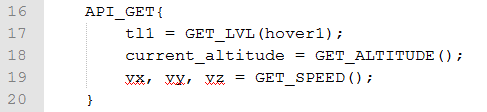
\includegraphics[width=0.7\textwidth]{img/apiget.png}
            \end{center}
\end{figure}

\section{Exemple récapitulatif}

Voici un exemple d'automate, avec quelques explications.
\begin{center}
	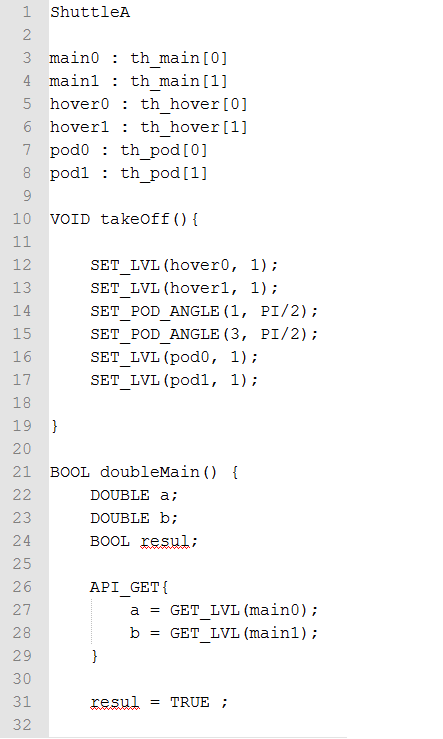
\includegraphics[scale=0.75]{img/otto1.png}
\end{center}

Comme prévu, l'initialisation de l'automate des lignes 1 à 8. Ensuite on définit une fonction VOID (qui ne renvoie pas de valeur) takeOff() qui oriente les boosters et met tous les systèmes de propulsion à 100\% de leur capacité (sauf les réacteurs principaux, à poussée horizontale). 


\begin{center}
	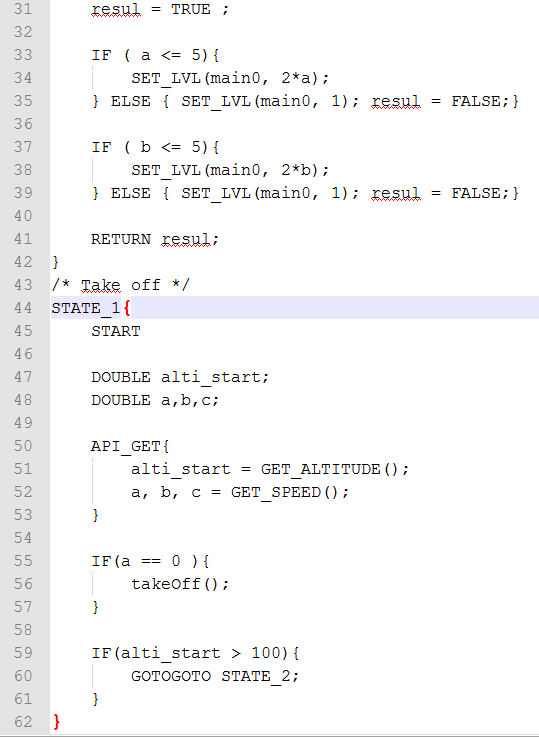
\includegraphics[scale=0.75]{img/otto2.png}
\end{center}
doubleMain() double la puissance délivrée par les réacteurs principaux, si ils sont à moins de 50\%, les met à 100\% sinon. Elle renvoie faux si le pourcentage de puissance n'a pas pu être doublée : c'est à dire si les réacteurs étaient déjà à plus de 50\% de leur capacité maximale. C'est une fonction illustrative, elle n'est d'ailleurs même pas utilisée.

Ensuite on définit l'état 1 comme état initial : \texttt{STATE\_1 \{ START [...] \} }
On définit des variables, et on leur donne des valeurs grâces aux fonctions de l'API.

\begin{center}
	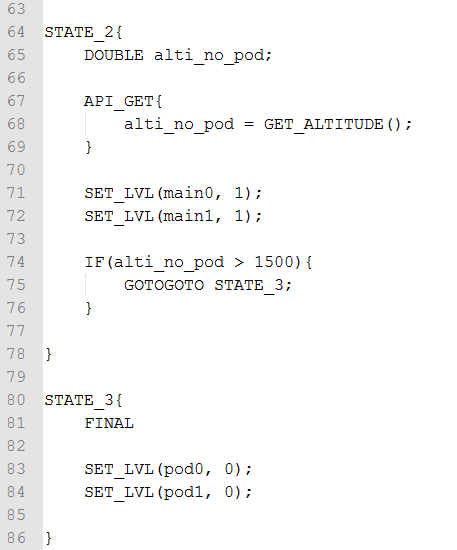
\includegraphics[scale=0.75]{img/otto3.png}
\end{center}

Dans le deuxième état on active les réacteurs principaux à 100\% de leur capacité.
Lorsque l'on atteint 1500m d'altitude, on passe à l'état 3. Celui ci coupe les booster.

%%%%%%%%%%%%%%%%%%%%%%%%%%%%%%%%%%%%%%%%%%%%%%%%%%%%%%%%%%%%%%%%%%%%%%%%%%%%%%%
\section{Compilation}

Voici un récapitulatif des étapes et instructions nécessaires pour rendre votre automate pleinement fonctionnel. Cette partie s'adresse aux utilisateurs qui n'utilisent pas le script python pour tout compiler automatiquement.

\subsection{Compiler le compilateur}
\onehalfspacing 

Dans un premier temps, vous devrez compiler le compilateur java. Il s'agira donc de se placer dans le dossier où est placé le compilateur, c'est-à-dire le dossier grammar, pour démarrer la compilation grâce à ant.

\begin{itemize}
	\item Se placer dans le dossier "grammar" :	
	\begin{itemize}
					\item Démarrer -> Accessoires -> Invite de commande
					\item Saisir la commande cd et coller l'emplacement du dossier grammar 
	\end{itemize}
\end{itemize}

Attention les étapes suivantes nécessitent d'avoir javaCC et ant installés, et ajoutés dans le PATH.

\begin{itemize}
	\item Dans la fenêtre de l'invite de commande, saisir ant grammar
	\item Saisir ant compile
\end{itemize}
		
\begin{center}
	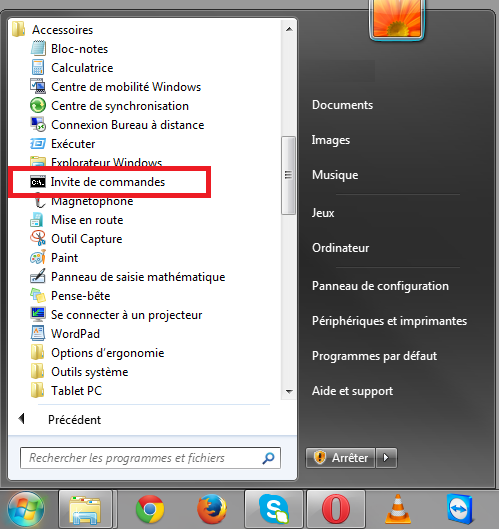
\includegraphics[scale=0.75]{img/cmd.png}
\end{center}


\subsection{Compiler un automate}
La première tâche pour compiler l'automate est bien sûr de l'écrire, puis de le donner en argument au compilateur Mittlewerk.\newline

\begin{itemize}
	\item Ecrire un automate, par exemple dans un fichier toto.mw (le nom n'a pas dimportance, l'extension non plus, pourvu que le texte soit brut)
	\begin{itemize}
					\item Démarrer -> Accessoires -> Invite de commande
					\item Saisir la commande cd et coller l'emplacement du dossier grammar \newline
	\end{itemize}
	
	\item Dans la fenêtre de l'invite de commande, saisir : java -cp class Core.Mittelwerk toto.mw <optional\_output.cpp> <optional\_output.h>
	\item <optional\_output.cpp> contient le code de l'automate
	\item <optional\_output.h> contient le code à coller dans le header du vaisseau	
\end{itemize}


\subsection{Compiler les dll du vaisseau}

Le code étant généré hors des fichiers du vaisseau, il va falloir l'intégrer dans les fichiers sources de celui-ci.
On suppose que le code est généré dans "Otto.cpp" et "header.h", (attention : la procédure n'est valide que pour le Shuttle A).\newline
\begin{itemize}
	\item Ouvrir le projet Visual studio du vaisseau
	\item Ajouter le fichier "Otto.cpp" dedans
	\item Trouver la fonction clbkPostStep dans le code du vaisseau
	\begin{itemize}
		\item Ajouter en toute première ligne de cette fonction : 
		\item postStep(simt, simdt, mjd);
	\end{itemize}
	\item Aller dans le header du vaisseau (ShuttleA.h), dans la section privée :
	\begin{itemize}
		\item Coller le contenu de "header.h" (précédemment généré) dedans.
	\end{itemize}
	
\end{itemize}

\end{document}




%%%%%%%%%%%%%%%%%%%%%%%%%%%%%%%%%%%%%%%%%%%%%%%%%%%%%%%%%%%%%%%%%%%%%%%%%%%%%%%
